\documentclass{article}
\usepackage[utf8]{inputenc}
\usepackage{polski}
\usepackage{geometry}
\usepackage{pdfpages}
\usepackage{pdfpages}
\usepackage{listings}
\usepackage{listingsutf8}
\usepackage{multirow}
\usepackage{siunitx}
\usepackage{multirow}
\usepackage{booktabs}
\usepackage{tabularx}
\usepackage{placeins}
\usepackage{pdflscape}
\usepackage{graphicx}
\usepackage{subfig}
\usepackage{hyperref}
\usepackage{amsmath}
\usepackage{colortbl}

\geometry{
a4paper,
total={170mm,257mm},
left=20mm,
top=20mm
}
\newcolumntype{Y}{>{\centering\arraybackslash}X}
% \renewcommand\thesection{}
\lstset{%
literate=%
 {ą}{{\k{a}}}1
 {ę}{{\k{e}}}1
 {Ą}{{\k{A}}}1
 {Ę}{{\k{E}}}1
 {ś}{{\'{s}}}1
 {Ś}{{\'{S}}}1
 {ź}{{\'{z}}}1
 {Ź}{{\'{Z}}}1
 {ń}{{\'{n}}}1
 {Ń}{{\'{N}}}1
 {ć}{{\'{c}}}1
 {Ć}{{\'{C}}}1
 {ó}{{\'{o}}}1
 {Ó}{{\'{O}}}1
 {ż}{{\.{z}}}1
 {Ż}{{\.{Z}}}1
 {ł}{{\l{}}}1
 {Ł}{{\l{}}}1
}

\title{Metody Programowania Równoległego\\ Raport II - Pętla for}
\author{Samuel Hełdak, Maciej Trątnowiecki}
\date{AGH, Semestr Letni, 2022}

\begin{document}
    \maketitle
    \lstset{ 
      backgroundcolor=\color{white},   % choose the background color; you must add \usepackage{color} or \usepackage{xcolor}; should come as last argument
      basicstyle=\footnotesize,        % the size of the fonts that are used for the code
      breakatwhitespace=false,         % sets if automatic breaks should only happen at whitespace
      breaklines=true,                 % sets automatic line breaking
      captionpos=b,                    % sets the caption-position to bottom
      commentstyle=\color{mygreen},    % comment style
      deletekeywords={...},            % if you want to delete keywords from the given language
      escapeinside={\%*}{*)},          % if you want to add LaTeX within your code
      %extendedchars=true,              % lets you use non-ASCII characters; for 8-bits encodings only, does not work with UTF-8
      firstnumber=1000,                % start line enumeration with line 1000
      frame=single,	                   % adds a frame around the code
      keepspaces=true,                 % keeps spaces in text, useful for keeping indentation of code (possibly needs columns=flexible)
      keywordstyle=\color{blue},       % keyword style
      language=Octave,                 % the language of the code
      morekeywords={*,...},            % if you want to add more keywords to the set
      numbers=left,                    % where to put the line-numbers; possible values are (none, left, right)
      numbersep=5pt,                   % how far the line-numbers are from the code
      numberstyle=\tiny\color{mygray}, % the style that is used for the line-numbers
      rulecolor=\color{black},         % if not set, the frame-color may be changed on line-breaks within not-black text (e.g. comments (green here))
      showspaces=false,                % show spaces everywhere adding particular underscores; it overrides 'showstringspaces'
      showstringspaces=false,          % underline spaces within strings only
      showtabs=false,                  % show tabs within strings adding particular underscores
      stepnumber=2,                    % the step between two line-numbers. If it's 1, each line will be numbered
      stringstyle=\color{mymauve},     % string literal style
      tabsize=2,	                   % sets default tabsize to 2 spaces
      title=\lstname                   % show the filename of files included with \lstinputlisting; also try caption instead of title
    }
    % \lstinputlisting[language=bash]{no_qos.txt}
        % \begin{center}
        %     \includegraphics[width=13cm]{lab2/report/ex3_1.png}
        % \end{center}\\
        
    \section{Implementacja równoległego generowania losowych danych wejściowych}
        \subsection{Definicja problemu}
        W ramach zadania przygotowaliśmy implementację programu generującego równolegle losowe dane wejściowe dla algorytmu sortującego. Implementacja przygotowana została w języku C, za wykorzystaniem interfejsu \textit{OpenMP}. Kod implementacji dla poszczególnych wersji programu załączono w ostatniej sekcji sprawozdania. \\
        Tak przygotowany program wykorzystaliśmy do pomiaru czasu wykonania i przyśpieszenia algorytmu, dla różnych ustawień klauzuli \textit{schedule}.
    
        \subsection{Pomiary i wyniki}
        Każdy z pomiarów powtórzyliśmy dziesięciokrotnie dla danych ustawień parametrów programu. Program testowaliśmy dla ustawień klauzuli \textit{schedule} ze zbioru \textit{guided}, \textit{dynamic} i \textit{static}, oraz wartości parametru \textit{chunk} z zakresu opisanego w tabeli poniżej.  
        
        \begin{center}
            \begin{table}[ht]
                \centering
                \begin{tabular}{|c|c|c|}
                    \hline
                    Schedule  & Chunk\\
                    \specialrule{1pt}{1pt}{1pt}
                    Dynamic & 1 \\
                    Dynamic & 1000\\
                    Dynamic & Rozmiar Problemu / Ilość CPU \\
                    Guided & 1\\
                    Static & Rozmiar Problemu / Ilość CPU \\
                    \hline
                \end{tabular}
                \caption{Parametry programu wykorzystane do przygotowania pomiarów.}
            \label{tab:my_label}
            \end{table}
        \end{center}
        Program uruchamialiśmy dla problemów o rozmiarze $10^6$, $10^7$ i $10^8$. Zebrane wyniki pomiarów czasu wykonania programu przedstawione zostały na poniższych wykresach.
        
        \newpage
        \begin{figure}[h!]
            \centering
            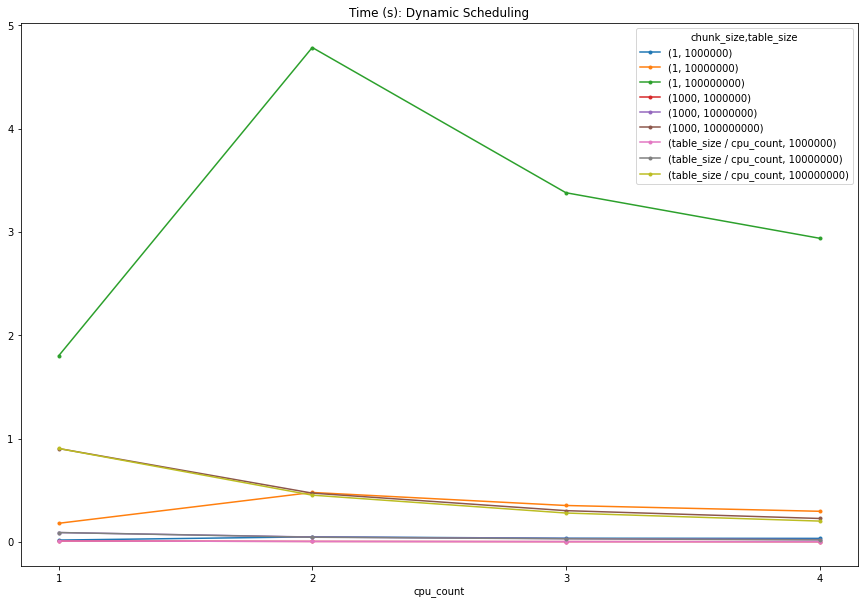
\includegraphics[width=17cm]{report2/images/Type/ex3_dynamic_mean.png}
            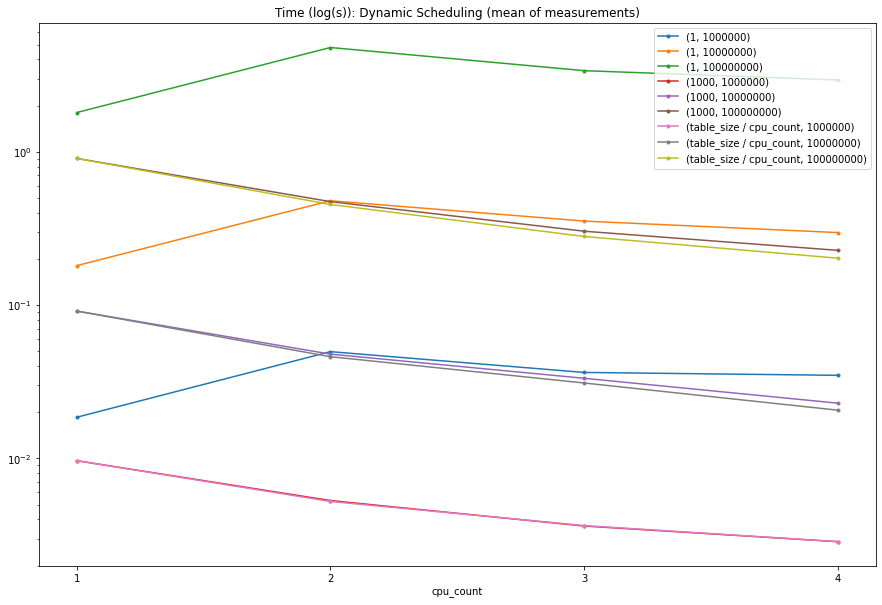
\includegraphics[width=17cm]{report2/images/Type/ex3_dynamic_mean_log.png}
            \caption{Pomiar czasu wykonania programu, Dynamic schedule, w zależności od parametrów. Uśrednione wartości z powtórzeń pomiarów. }
        \end{figure}
        \begin{figure}[h!]
            \centering
            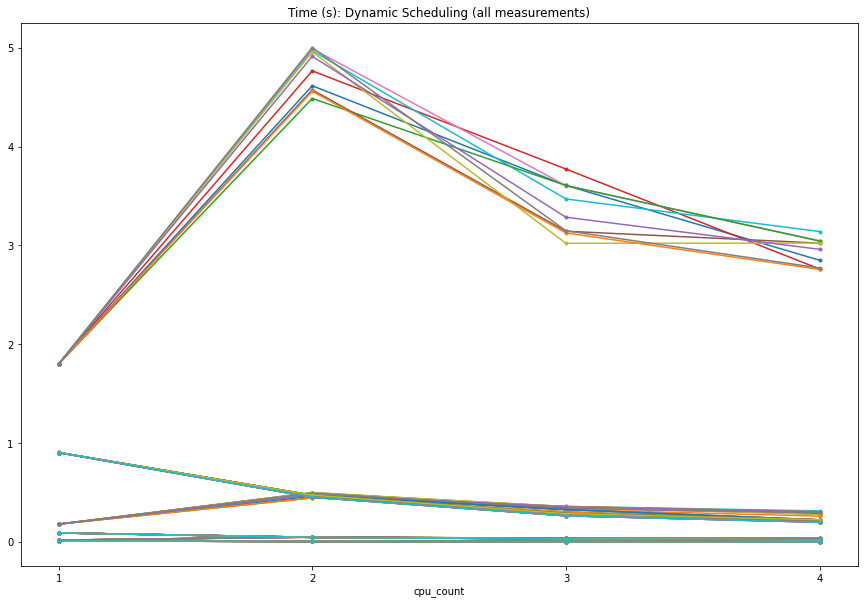
\includegraphics[width=17cm]{report2/images/Type/ex3_dynamic_all.png}
            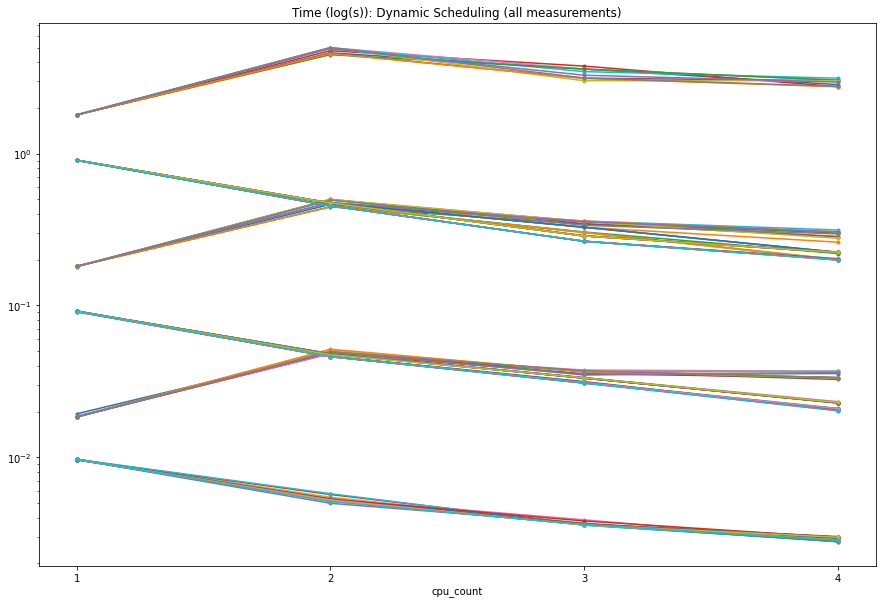
\includegraphics[width=17cm]{report2/images/Type/ex3_dynamic_all_log.png}
            \caption{Pomiar czasu wykonania programu, Dynamic schedule. Wszystkie pomiary. }
        \end{figure}
        \newpage
        \begin{figure}[h!]
            \centering
            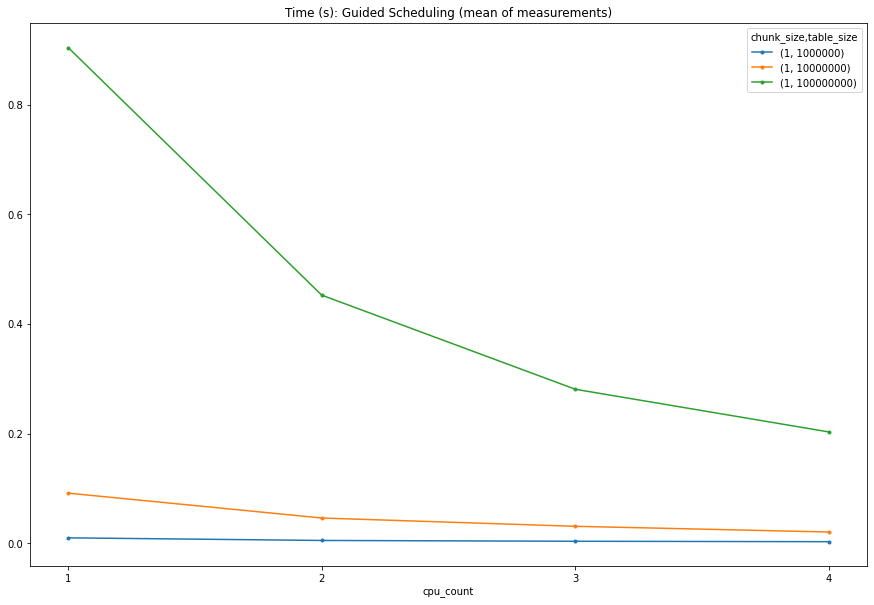
\includegraphics[width=17cm]{report2/images/Type/ex3_guided_mean.png}
            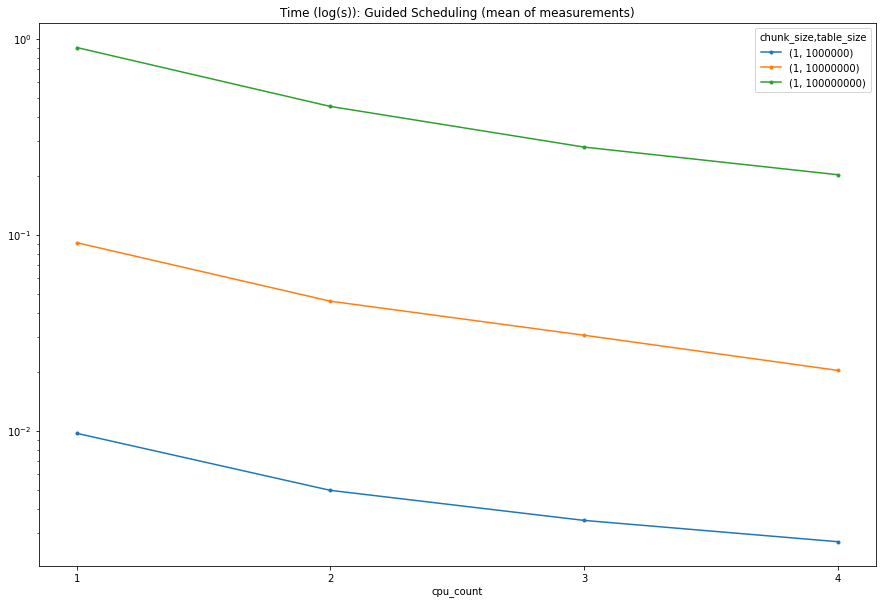
\includegraphics[width=17cm]{report2/images/Type/ex3_guided_mean_log.png}
            \caption{Pomiar czasu wykonania programu, guided schedule, w zależności od parametrów. Uśrednione wartości z powtórzeń pomiarów. }
        \end{figure}
        \newpage
        \begin{figure}[h!]
            \centering
            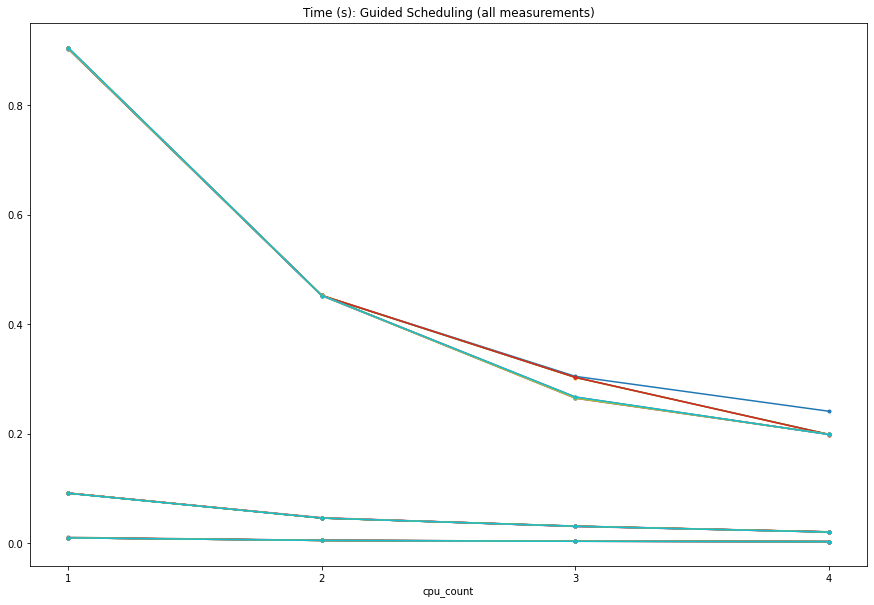
\includegraphics[width=17cm]{report2/images/Type/ex3_guided_all.png}
            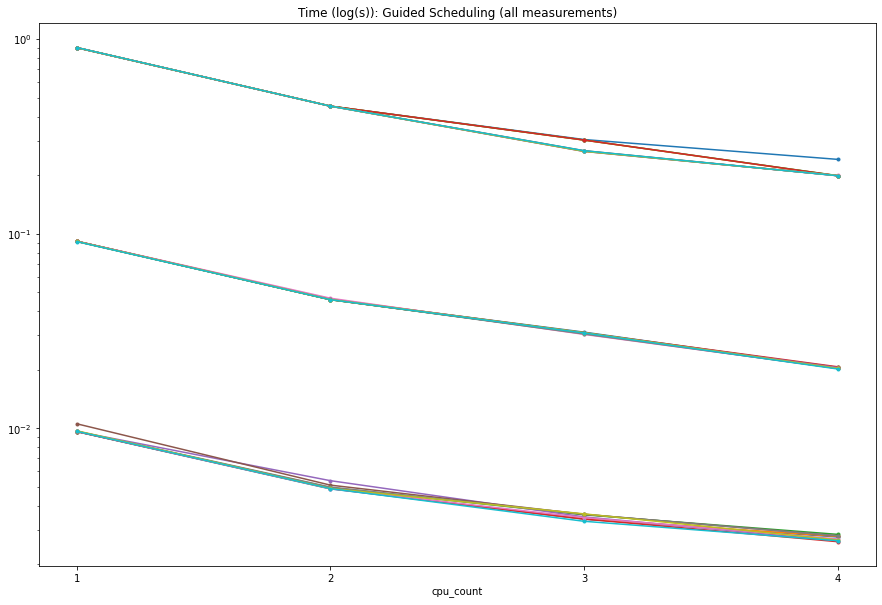
\includegraphics[width=17cm]{report2/images/Type/ex3_guided_all_log.png}
            \caption{Pomiar czasu wykonania programu, guided schedule. Wszystkie pomiary. }
        \end{figure}
        \newpage
        \begin{figure}[h!]
            \centering
            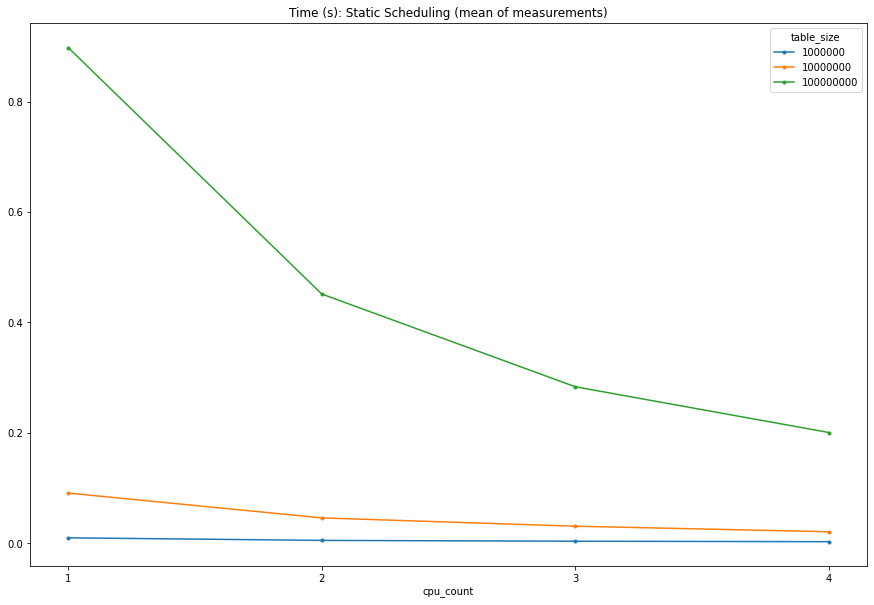
\includegraphics[width=17cm]{report2/images/Type/ex3_static_mean.png}
            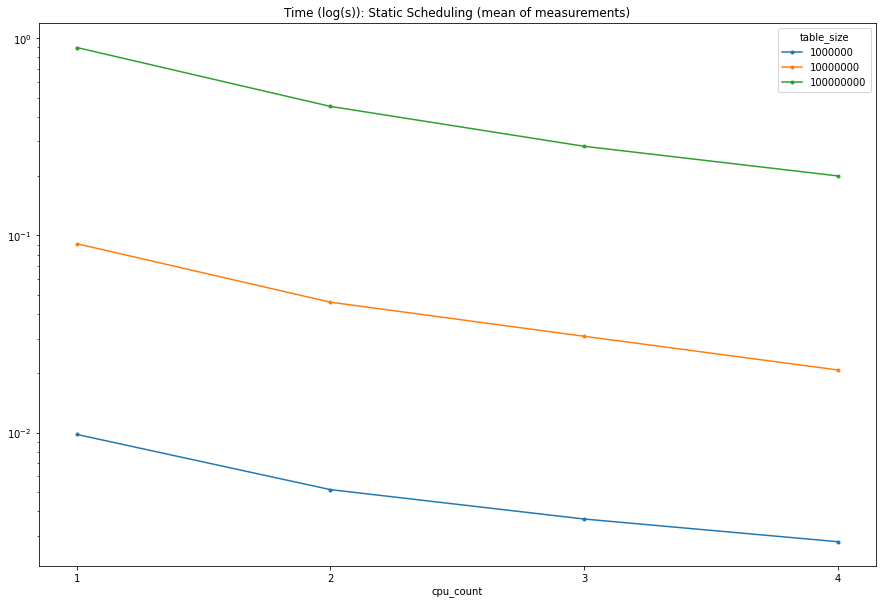
\includegraphics[width=17cm]{report2/images/Type/ex3_static_mean_log.png}
            \caption{Pomiar czasu wykonania programu, static schedule, w zależności od parametrów. Uśrednione wartości z powtórzeń pomiarów. }
        \end{figure}
        \newpage
        \begin{figure}[h!]
            \centering
            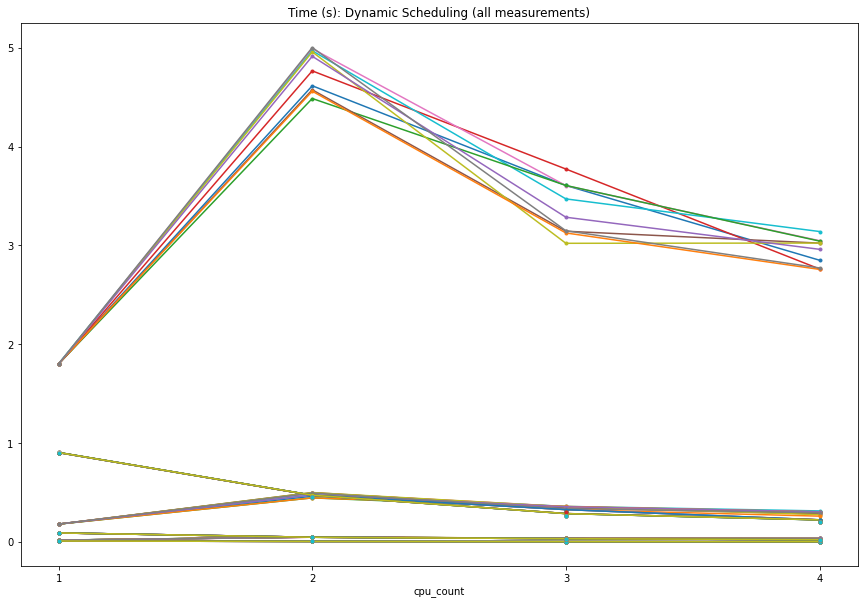
\includegraphics[width=17cm]{report2/images/Type/ex3_static_all.png}
            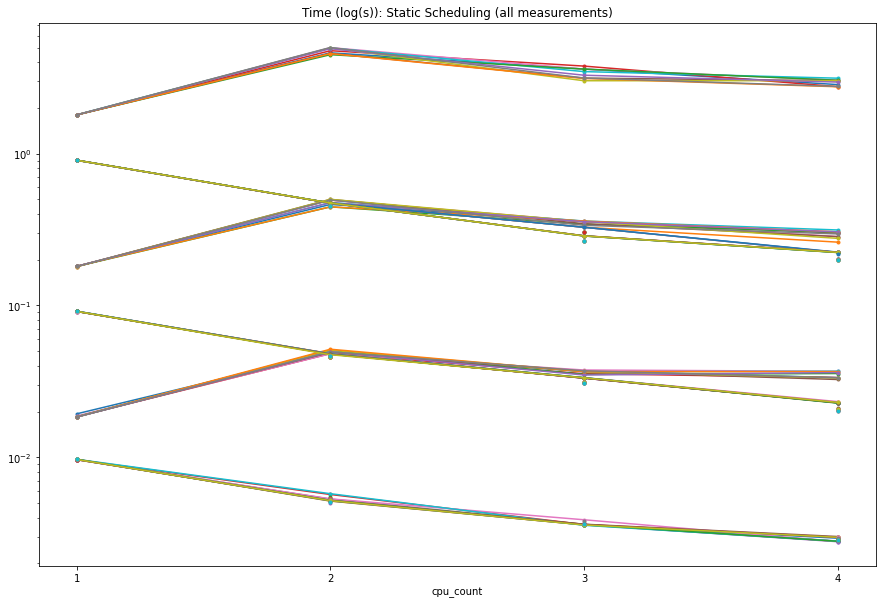
\includegraphics[width=17cm]{report2/images/Type/ex3_static_all_log.png}
            \caption{Pomiar czasu wykonania programu, static schedule. Wszystkie pomiary. }
        \end{figure}
        \newpage
        \begin{figure}[h!]
            \centering
            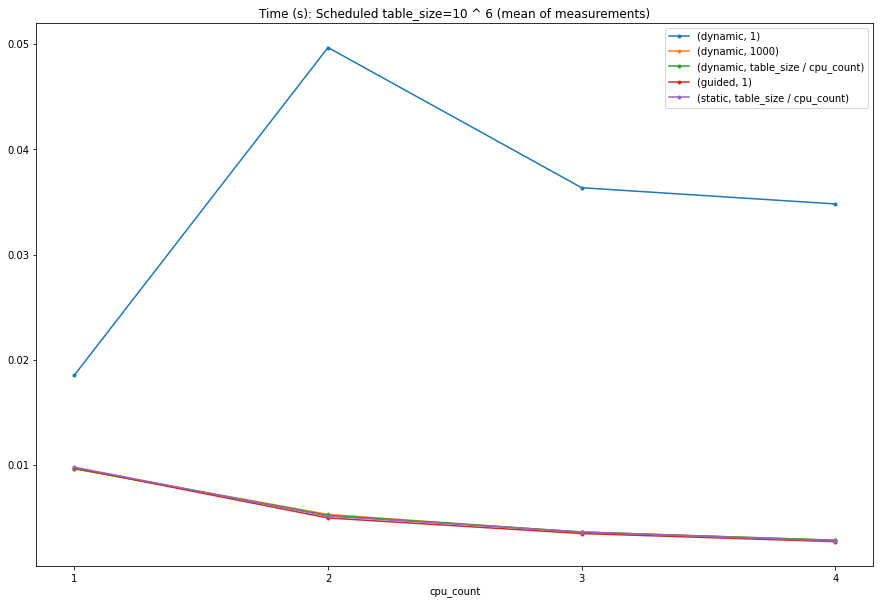
\includegraphics[width=17cm]{report2/images/TableSize/ex3_tb6_mean.png}
            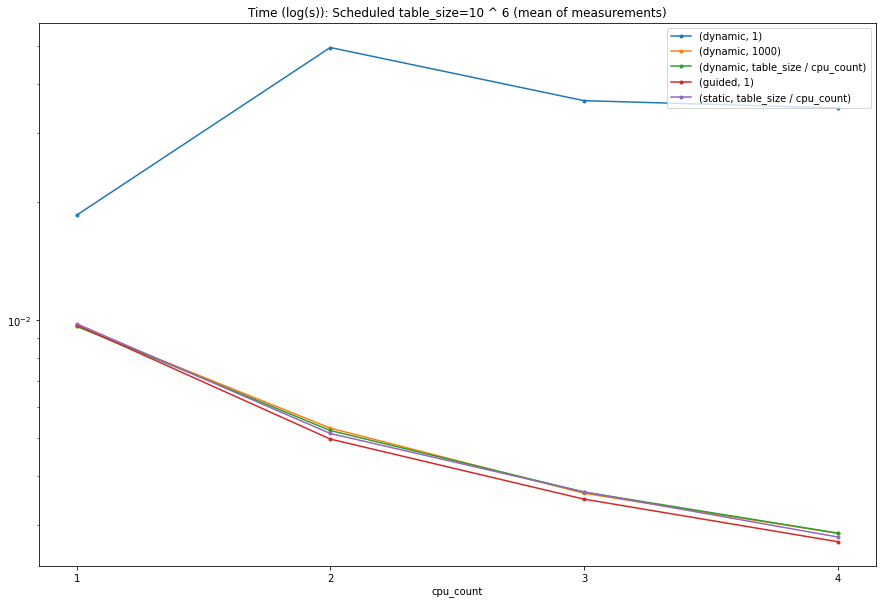
\includegraphics[width=17cm]{report2/images/TableSize/ex3_tb6_mean_log.png}
            \caption{Pomiar czasu wykonania programu, dla problemu rozmiaru 10 ** 6, w zależności od parametrów. Uśrednione wartości z powtórzeń pomiarów. }
        \end{figure}
        \newpage
        \begin{figure}[h!]
            \centering
            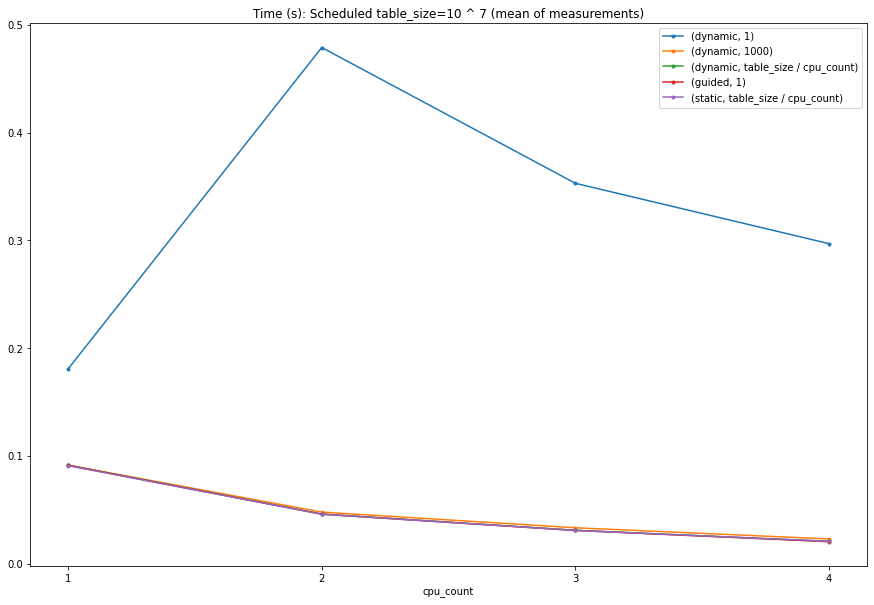
\includegraphics[width=17cm]{report2/images/TableSize/ex3_tb7_mean.png}
            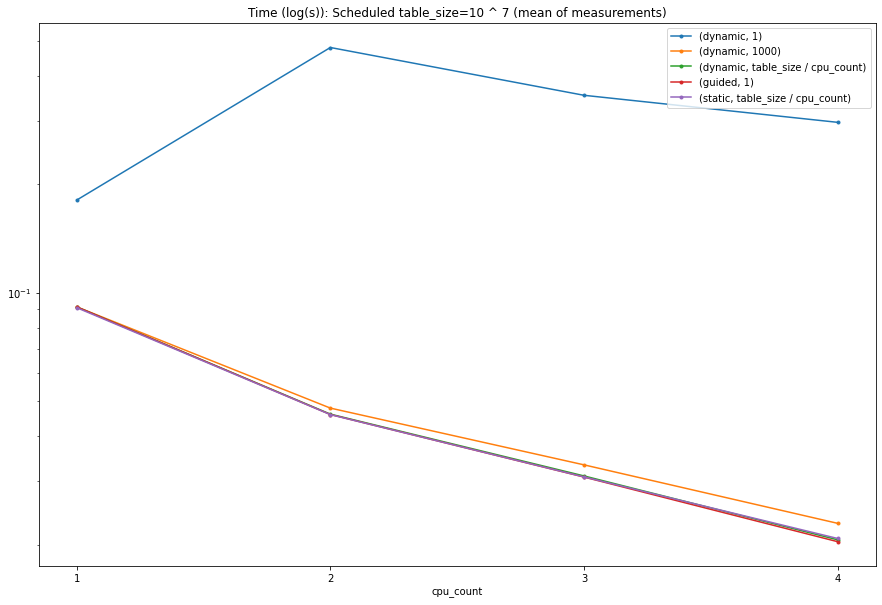
\includegraphics[width=17cm]{report2/images/TableSize/ex3_tb7_mean_log.png}
            \caption{Pomiar czasu wykonania programu, dla problemu rozmiaru 10 ** 7, w zależności od parametrów. Uśrednione wartości z powtórzeń pomiarów. }
        \end{figure}
        \newpage
        \begin{figure}[h!]
            \centering
            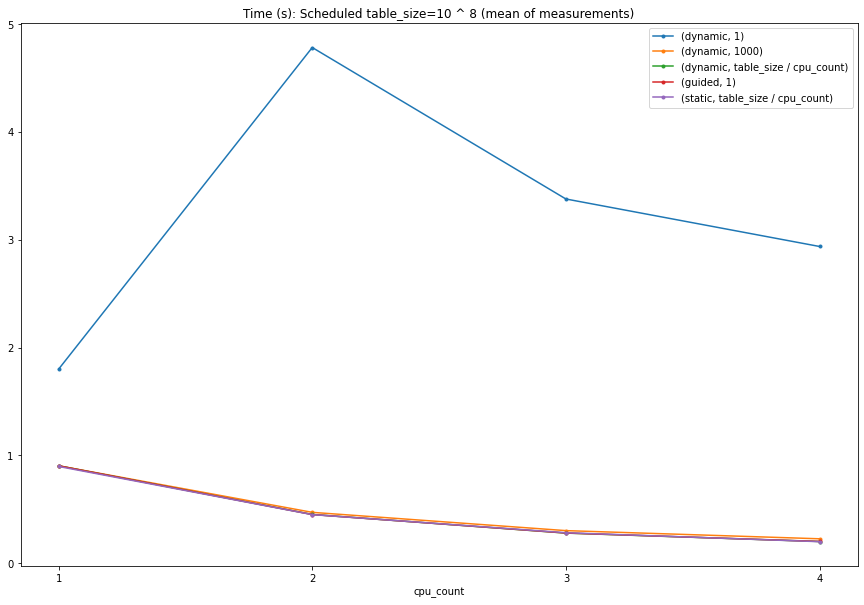
\includegraphics[width=17cm]{report2/images/TableSize/ex3_tb8_mean.png}
            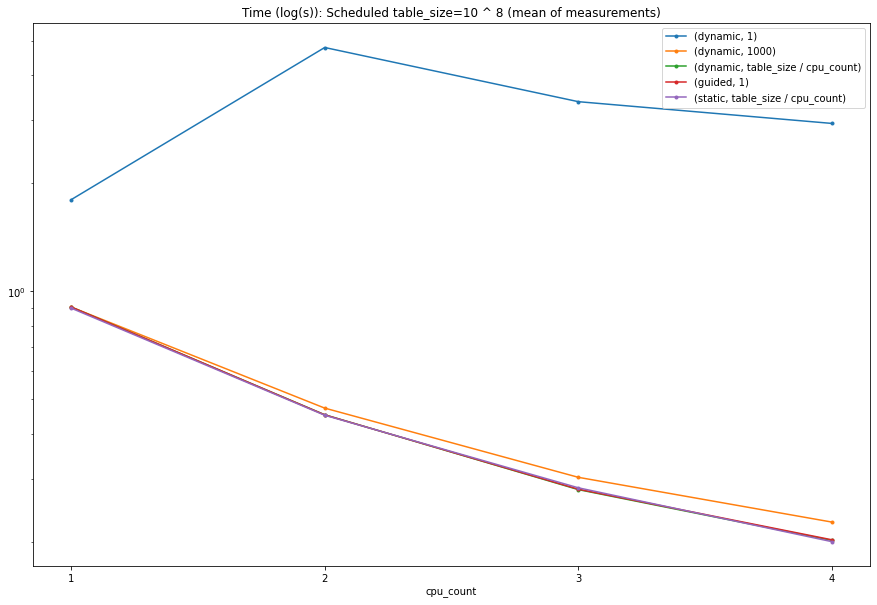
\includegraphics[width=17cm]{report2/images/TableSize/ex3_tb8_mean_log.png}
            \caption{Pomiar czasu wykonania programu, dla problemu rozmiaru 10 ** 8, w zależności od parametrów. Uśrednione wartości z powtórzeń pomiarów. }
        \end{figure}
        \newpage


        Na podstawie zmierzonych czasów pracy przygotowaliśmy także wykresy przyśpieszenia programu.
        \begin{figure}[h!]
            \centering
            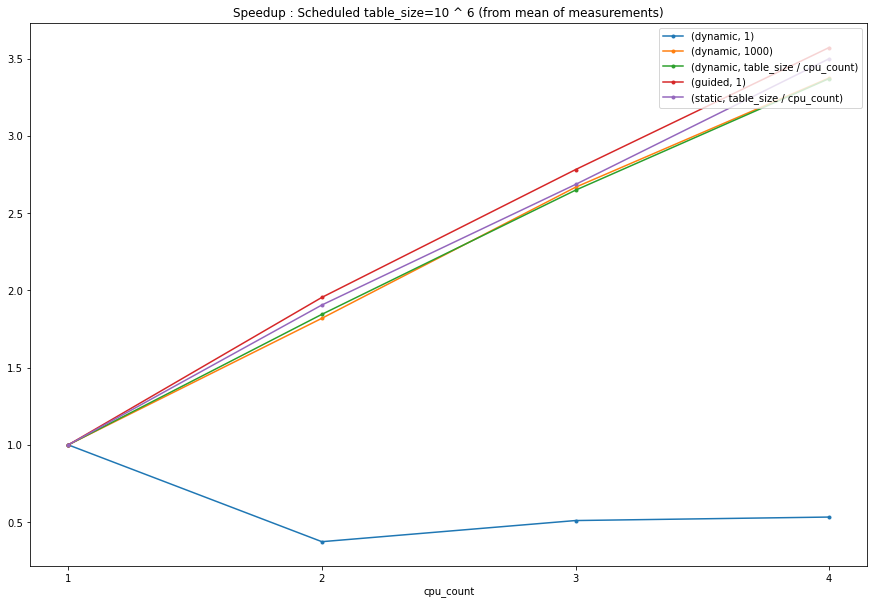
\includegraphics[width=17cm]{report2/images/TableSize/ex3_tb6_speedup.png}
            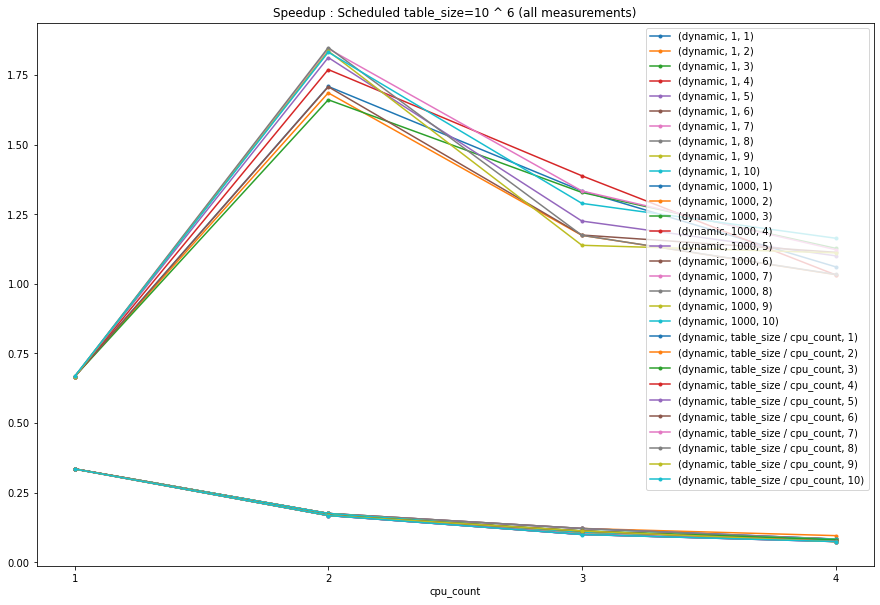
\includegraphics[width=17cm]{report2/images/TableSize/ex3_tb6_speedup_all.png}
            \caption{Pomiar przyśpieszenia czasu wykonania programu, dla problemu rozmiaru 10 ** 6, w zależności od parametrów. Uśrednione wartości z powtórzeń pomiarów. }
        \end{figure}
        \newpage
        \begin{figure}[h!]
            \centering
            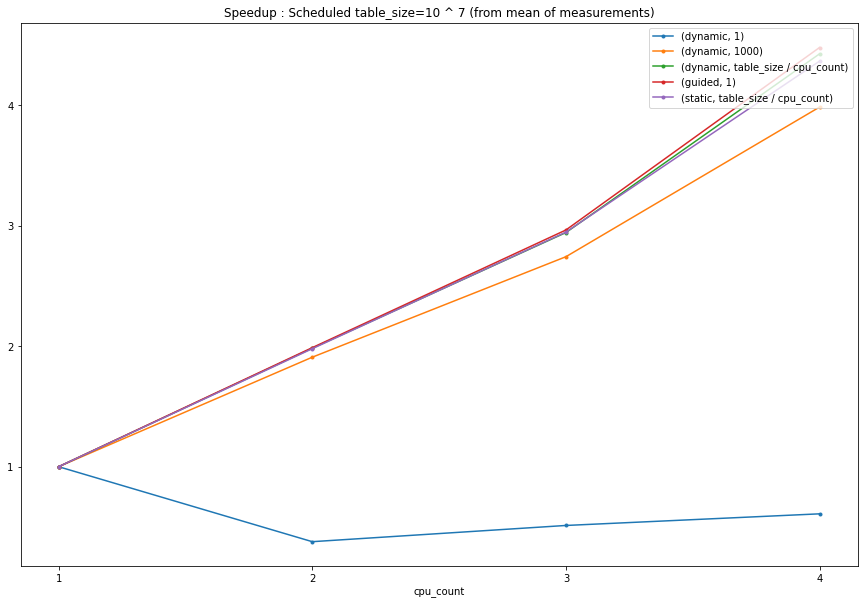
\includegraphics[width=17cm]{report2/images/TableSize/ex3_tb7_speedup.png}
            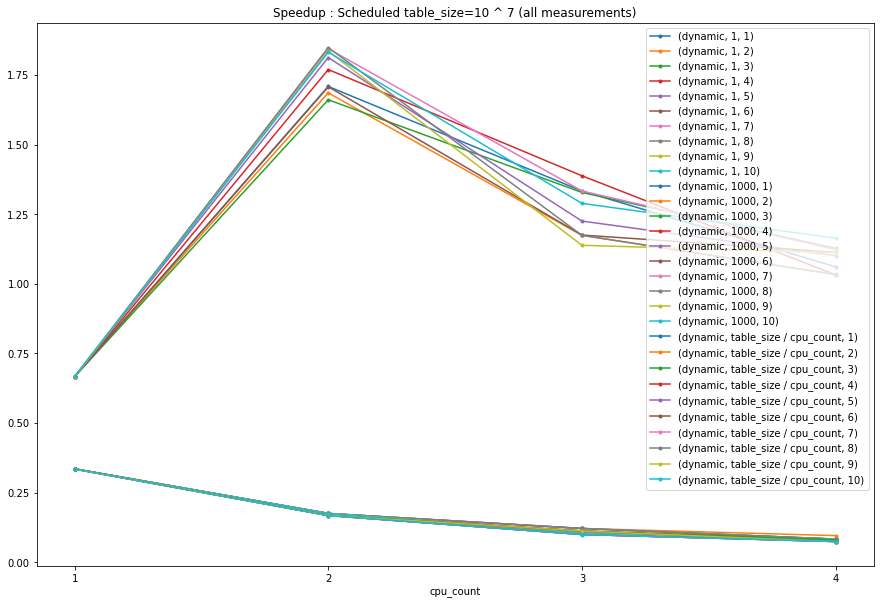
\includegraphics[width=17cm]{report2/images/TableSize/ex3_tb7_speedup_all.png}
            \caption{Pomiar przyśpieszenia czasu wykonania programu, dla problemu rozmiaru 10 ** 7, w zależności od parametrów. Uśrednione wartości z powtórzeń pomiarów. }
        \end{figure}
        \newpage
        \begin{figure}[h!]
            \centering
            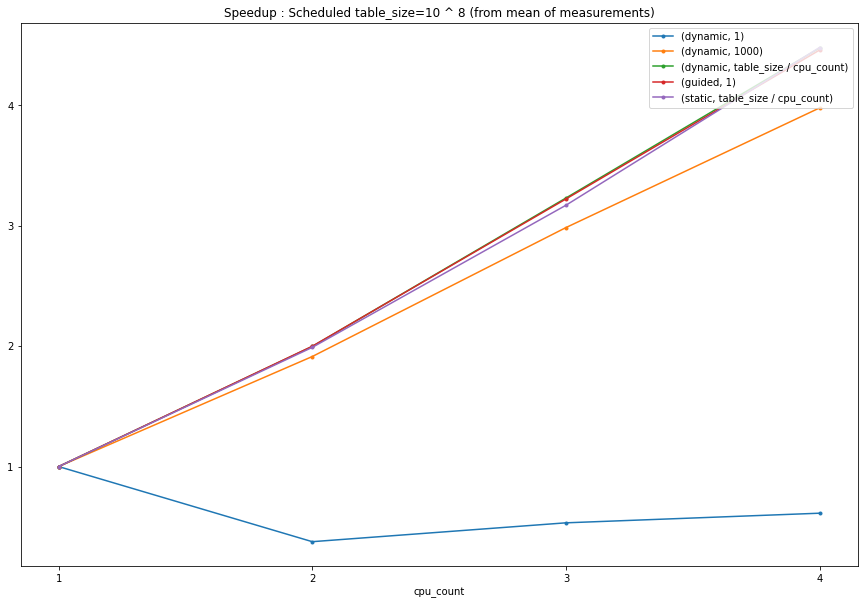
\includegraphics[width=17cm]{report2/images/TableSize/ex3_tb8_speedup.png}
            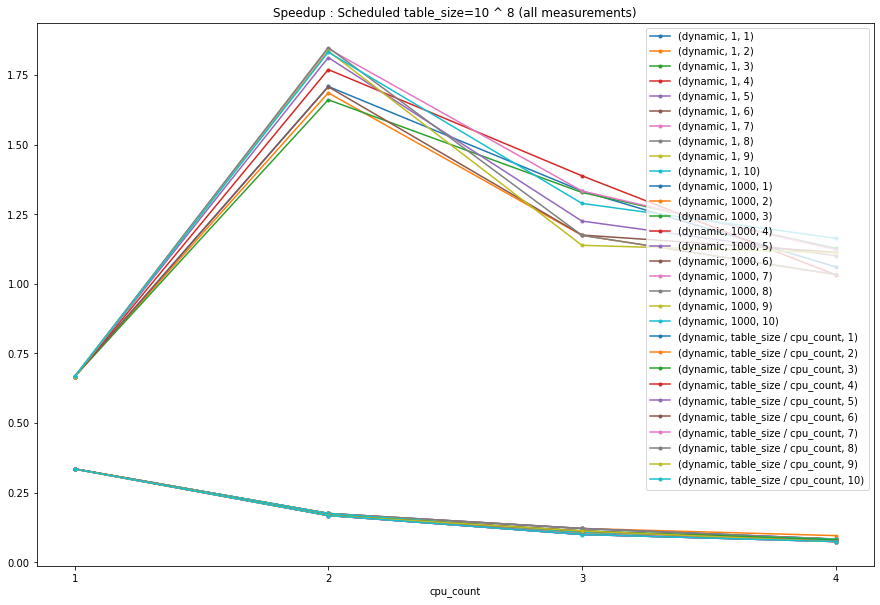
\includegraphics[width=17cm]{report2/images/TableSize/ex3_tb8_speedup_all.png}
            \caption{Pomiar przyśpieszenia czasu wykonania programu, dla problemu rozmiaru 10 ** 8, w zależności od parametrów. Uśrednione wartości z powtórzeń pomiarów. }
        \end{figure}


        \newpage
        \subsection{Wnioski}
        Analizując otrzymane wyniki pomiarów, zauważyć możemy że każda z typów klauzuli \textit{schedule} pozwoliła na uzyskanie zadowalających i porównywalnych przyśpieszeń, pod warunkiem wybrania odpowiedniej wartości parametru \textit{chunk}. W szczególności, klauzula \textit{guided} odpowiednio radzi sobie z jego dobraniem. Zauważyć możemy znaczny spadek wydajności, w przypadku wybrania zbyt małej wartości tego parametru dla wersji \textit{dynamic}, skutkującego nawet obniżeniem wydajności programu pomimo większej liczby dostępnych procesorów. 
        
        % \newpage
        \subsection{Kod programu}
        \lstinputlisting[language=c]{../ex3/schedule_static.c}
        \lstinputlisting[language=c]{../ex3/schedule_dynamic.c}
        \lstinputlisting[language=c]{../ex3/schedule_guided.c}
\end{document}
